%!TEX root = ../../report.tex
\subsection{Scenarios}
\copied{Scenarios : The description of an architecture is illustrated using a small set of use cases, or scenarios which become a fifth view. The scenarios describe sequences of interactions between objects, and between processes. They are used to identify architectural elements and to illustrate and validate the architecture design. They also serve as a starting point for tests of an architecture prototype. This view is also known as use case view.\\
	\\
	Scenarios are putting it all together. Interaction between objects in the
	system is expressed by object interaction and scenario diagrams as shown on
	Figure 6.
}
{from wikipedia\\\url{https://en.wikipedia.org/wiki/4\%2B1_architectural_view_model} and \url{http://pld.ttu.ee/~kruus/db_is02.pdf}}

This section describes the scenarios that are most likely to happen in our system. Scenarios are the interactions from our system with the different actors. First a textual step by step scenario is given, after that a diagram is shown with the scenario diagram.

\subsubsection*{Flood scenario}
\begin{enumerate}
  	\item The sensors monitor the water level
  	\item The algorithm requests weather forecast data
  	\item The weather forecast API returns the requested data
  	\item The algorithm sends a request to the UAV to validate results or provide extra images
  	\item The UAV provides the requested validation or extra images
  	\item The algorithm sends a warning to the warning part
  	\item The warning part requests the phone numbers from all subscribed citizens in the affected area
  	\item The database returns a list containing the corresponding phone numbers
  	\item The warning part invokes the emergency room API
  	\item The warning part invokes the SMS API, which sends a SMS to all phonenumbers on the list
\end{enumerate}

The different steps that are taken in the flood scenario are also represented in figure \ref{fig:flood-scenario}. This figure represents the logical connections that are made when a scenario is executed. This means that in reality a connection that is shown in the figure may not be made directly in reality. For example, the sensor data doesn't go directly from the sensors to the algorithm, there are some steps in between. 

\begin{figure}[H]
	%\centering
	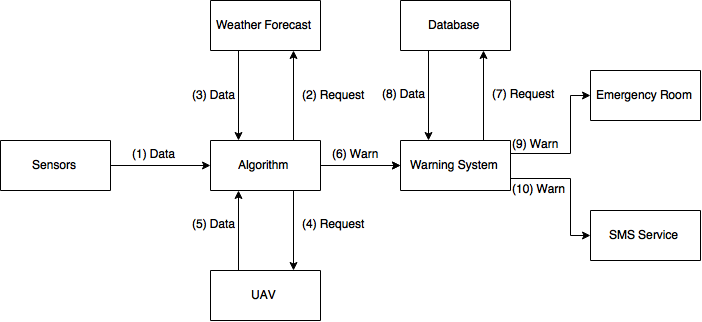
\includegraphics[keepaspectratio=true,width=0.9\textwidth]{{\viewimages/scenario1}.png}
	\caption{Scenario for a flood}
	\label{fig:flood-scenario}
\end{figure}

\subsubsection*{Guidance scenario}
\begin{enumerate}
	\item A citizen receives a warning text message
	\item A citizen requests guidance from a third party application to reach a safe area
	\item The third party application requests the current flood information from the third party API
	\item The third party API returns the requested data
	\item The third party application returns a route to a safe area
\end{enumerate}

When a flood is imminent or happening, a citizen can decide to request guidance to a safe area. If a citizen is subscribed to the SMS service, the citizen will get a warning text message in case of an imminent flood. Then the citizen can use a third party application that provides routes to safety that are as safe as possible.

\begin{figure}[H]
	%\centering
	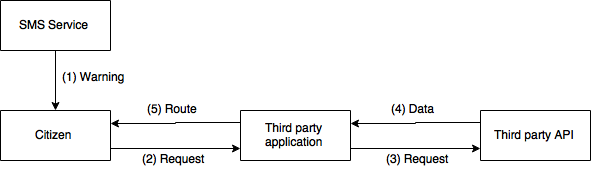
\includegraphics[keepaspectratio=true,width=0.9\textwidth]{{\viewimages/scenario2}.png}
	\caption{Scenario for guidance}
	\label{fig:guidance-scenario}
\end{figure}
